This chapter summarises the goals of the content profiling approach discussed so far and gives a detailed overview of the architecture for a prototype implementation of it. First a high level design is discussed and then detailed explanation of the chosen technology, implementation details, enhancements made and trade-offs is provided. Following some algorithms for representative sample selection that were implemented are presented and discussed. At the end a short summary and overview of future interesting work which will enhance the tool and help preservation experts even more in their endeavours is given.

\section{C3PO in Perspective}
As part of this thesis, a software prototype is developed that aims to tackle the issues, problems and gaps presented in the previous chapters. The aim is to create a tool that is able to automatically generate a content profile of large collections (consisting of hundreds of thousands, or even millions of objects). This means a framework that provides enough scalability to be feasibly applied on the metadata of collections of multi-terabyte ranges and beyond.

This profile includes a descriptive statistical representation of the content in the collection, meaning that it contains very specific data such as count of objects, overall size of objects, etc. Furthermore, it provides different visualisations of different aspects of the content, such as the file formats, mime types and many other characteristics and combinations thereof that are of interest to the user of the application.

As presented in section \ref{sec:goals} on page \pageref{sec:goals} the tool that implements the presented approach should fulfil the following requirements.

The user should be able to aggregate large sets of meta data with minimal effort in an automated fashion. The presented approach should be able to scale to million objects and should be ready to pass this threshold by making use of a distributed infrastructure and architecture.

Furthermore, clients of the application (users, or other systems) should be able to obtain a machine readable description of the profile, that contains enough information for the client to obtain a rough overview of the content at hand. This profile has to include the identifiers of a small set of objects that are representative to the whole collection as described in section \ref{sec:representative_sets} on page \pageref{sec:representative_sets}.

Since this overview might not be enough for a planning expert, she should be able to visualise interesting aspects of the content and filter it based on chosen characteristics. As it is unlikely that a single tool can satisfy all possible analysis requirements that an expert might have, it is very important that the raw data or a subset of it is exported in some intermediary format. This will allow further analysis conducted with other software, that might potentially result in even more interesting findings. 

%On top of that a service layer enables the user to query the tool in order to gain a deeper insight into the content. This may include the filtering of the content based on different characteristics and splitting it into buckets, which will allow to compare homogeneous parts (based on one or more characteristika) in an otherwise heterogenous content. 

%Visualizations and multi dimensional representations of these filterings enable to user to understand the profile and thus provide her with the fundamental knowledge and a more stable ground to take more efficient decisions.
The prototype implementation of the profiling approach is called '\textbf{C}lever, \textbf{C}rafty \textbf{C}ontent \textbf{P}rofiling of \textbf{O}bjects' or \textit{c3po} for short and is discussed in detail in the following subsections.
% idea
% overview
% part of scape, watch source, etc..

\section{Architecture}
In this section an overview of the architecture of c3po and its more important aspects are presented. Afterwards, detailed information about the design and implementation is given as well as a discussion of the decisions made is done. The implementation was carried out into two iterations which are presented after the overview.

\subsection{High Level Overview}
C3PO is separated into different modules and provides a relatively simple workflow that follows the three steps of content profiling as presented in \cite{petrov-ipres2012} and discussed in section \ref{sec:content_profiling} on page \pageref{sec:content_profiling}. In the first part it gathers raw meta data and parses it in order to normalise it into a simple internal data model. In the next step the data is cleaned up, partially aggregated and stored into an external to the tool database.
This offers the baseline for the deeper analysis provided by some of the modules in a stack diagram which is detailed in the following subsections.


\begin{figure}[htb]
\begin{center}
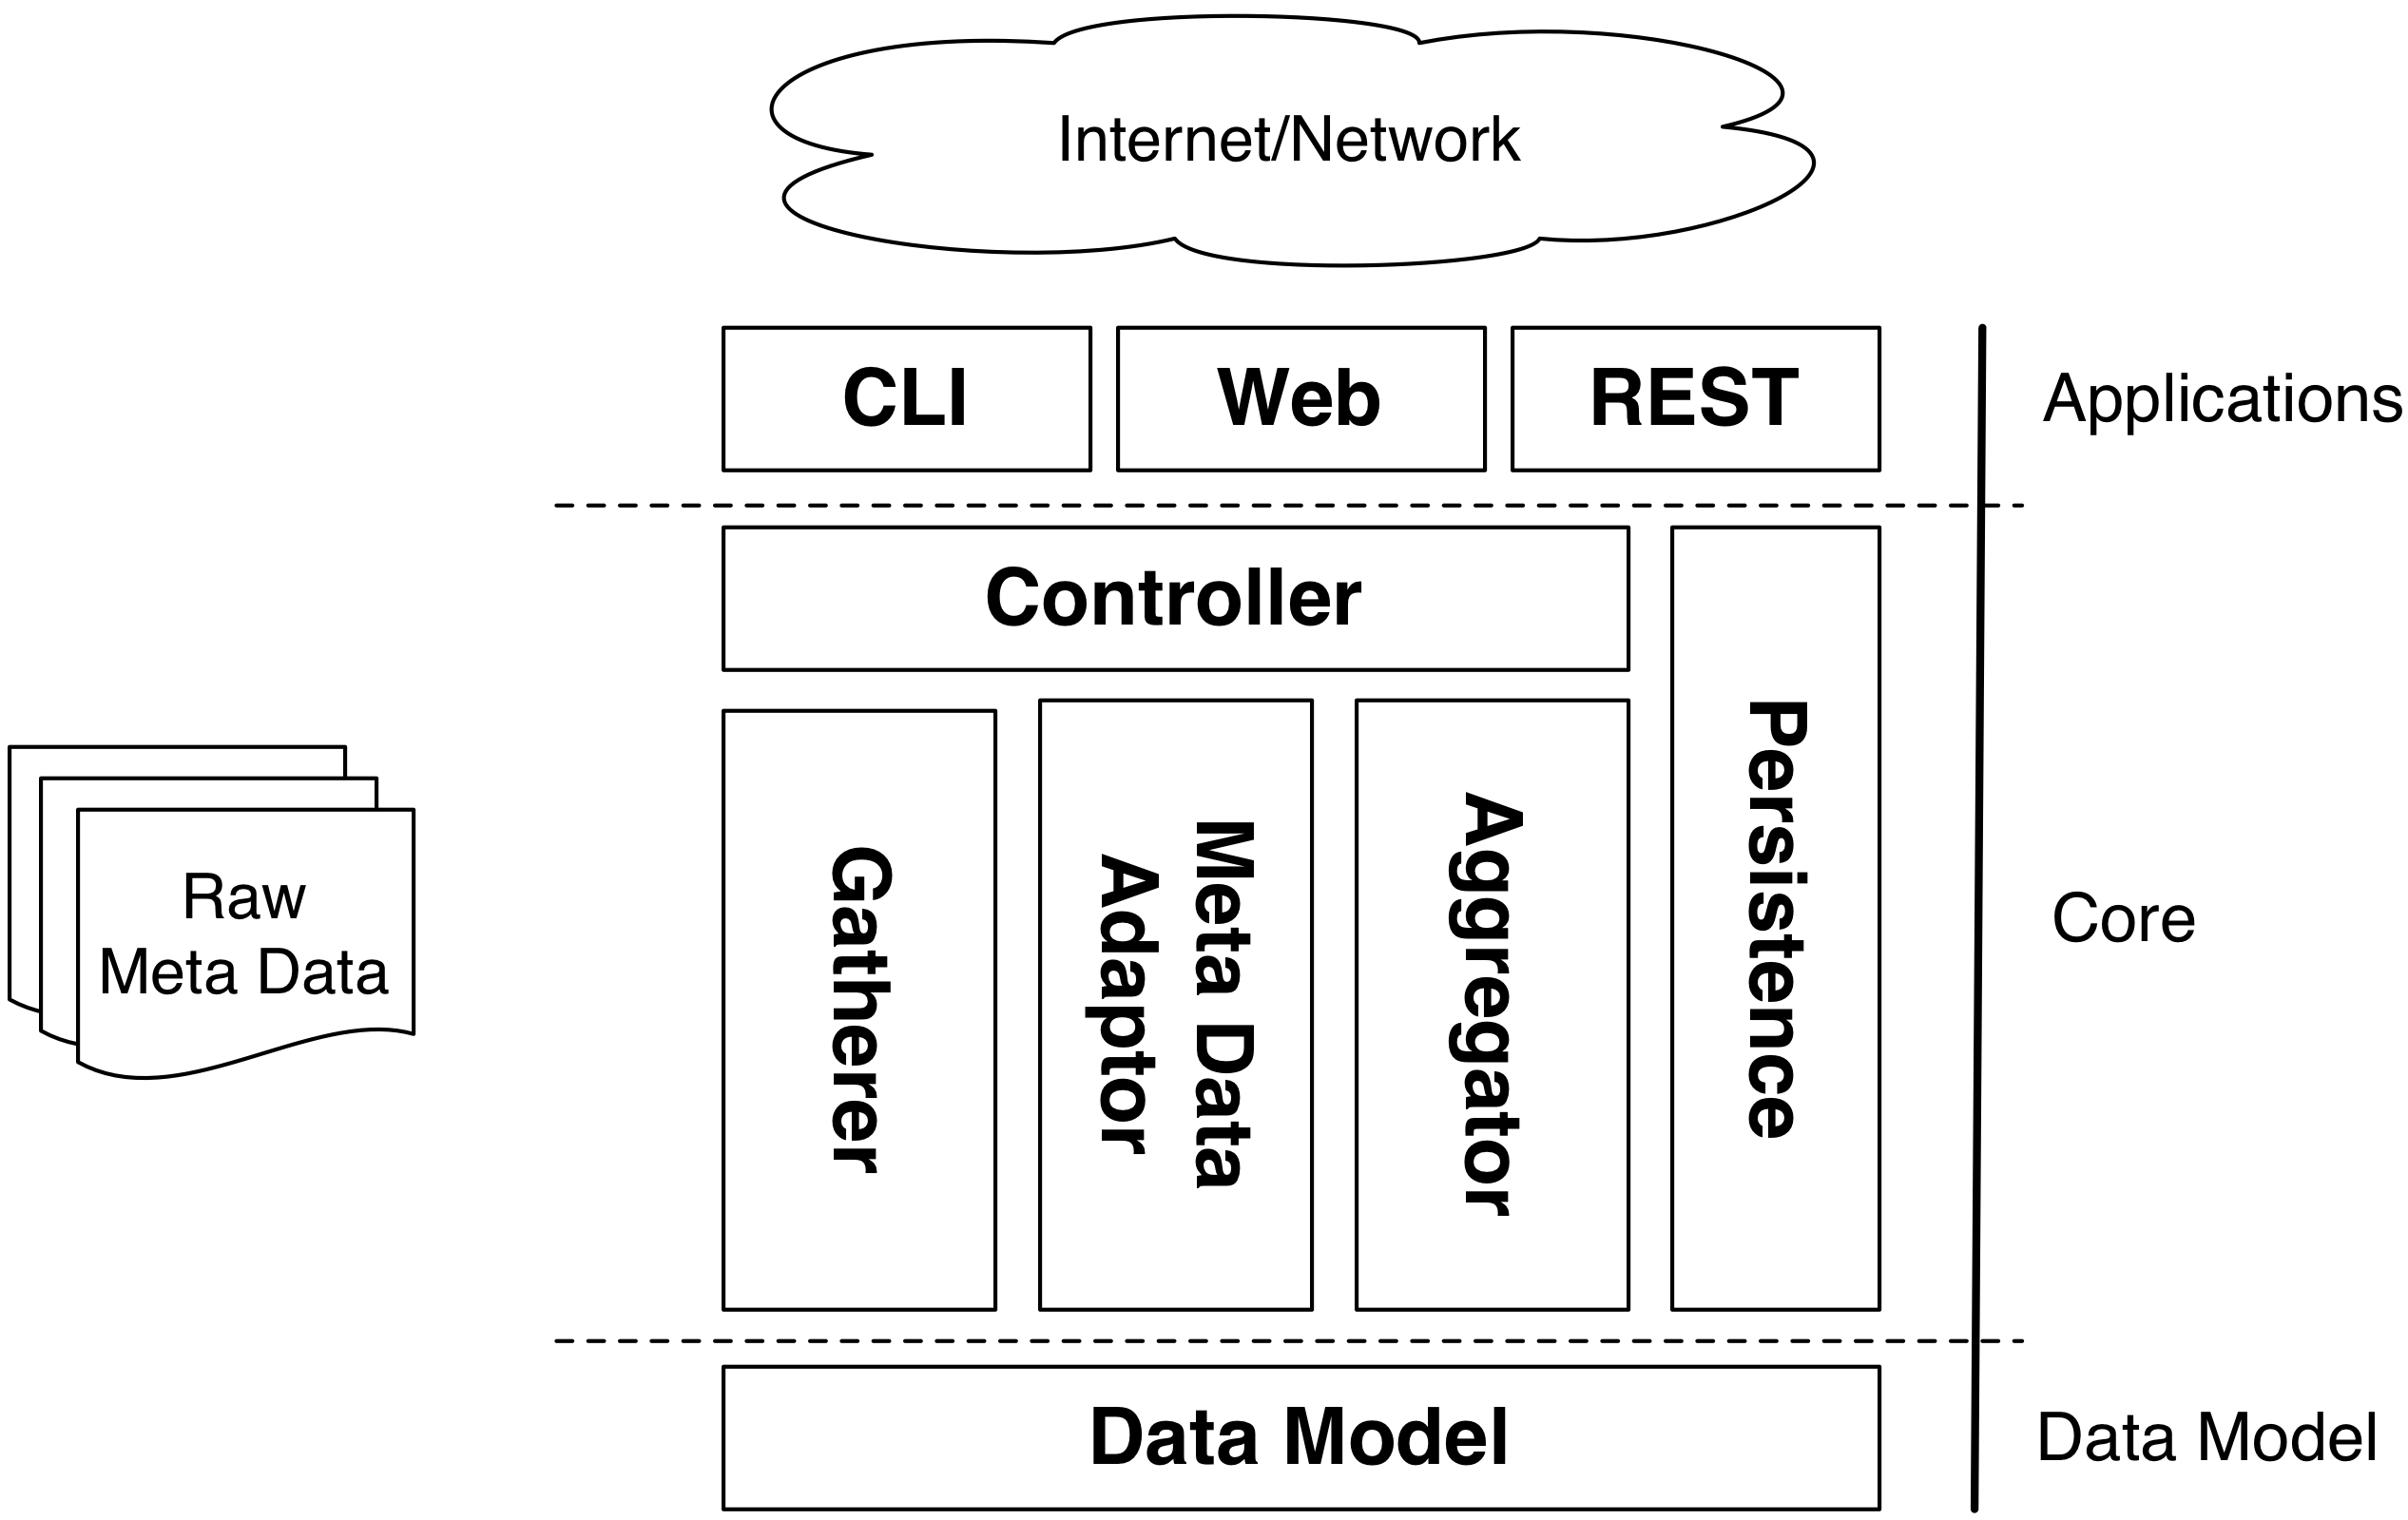
\includegraphics[width=5.5in]{figures/architecture/c3po_highlevel_architecture.png}
\caption{High-level architecture of c3po.}
\label{fig:architecture_highlevel}
\end{center}
\end{figure}

Figure \ref{fig:architecture_highlevel} presents the high level architecture and its modules.

\subsubsection{Data Model}

At the bottom there is the domain model module which sits as the foundation of the architecture. It represents a simple model that captures the important aspects of the content meta data in a generic way, but still provides the ability to do flexible queries over the data. It consists mainly of elements, properties and values. Elements encapsulate a digital object and capture important information, such as the identifier of an object within its source (e.g. a digital repository), which is important for later access. Properties define characteristics of a given object. These may include information, such as size, format, format version, etc. The values capture measurements of specific properties that are provided by different tools.

\subsubsection{Core}
Above the data model is the main part or the core module, which encapsulates the framework that allows the gathering, normalising and aggregation of the data. It not only offers interfaces that allow the extension of the framework, but also provides the glue-ware to create and run the work flow.

The core wraps the middle part of the architecture stack diagram. It is divided into three logical parts: A controller, sub-components and a persistence layer.

The controller is responsible for chaining the sub components and carrying out the whole workflow of the system.

The three sub-components (Gatherer, Meta Data Adaptor and Aggregator) divide the work and encapsulate important steps of the whole workflow. As described in section (TODO cite) the raw meta data of the content can be stored in many different places or sources. For example, it can be provided locally, in form of files stored on the local file system, or remotely. The remote source can have many different variations. E.g. there can be a remote ssh server that stores the raw meta data again in file form, or a remote web archive server that stores the meta data in special container files called arc (archive) or warc (web archive) file, but there can be also a remote repository, which not only stores the original content but all the meta data for each object in a different way (internal data store, to its local file system, etc.). The latter represents the most likely use case in a real world digital preservation scenario, however all others are possible as well, not to mention that they are easier to use for experimentation purposes.

As the users of c3po should not be interested in the way of how and where the meta data is stored, the gatherer component offers an interface that abstracts this issue.

Since different sources can use different characterisation tools and different characterisation tool outputs, the Meta Data Adaptor component is responsible for instantiating and assigning a specific implementation of an adaptor that can handle the gathered meta data records. 

The last part of the core module is the persistence layer, which abstracts the connection to the external data source, where all raw meta data is stored. It provides interfaces for retrieving the meta data, storing aggregations and analysis results.

\subsubsection{Applications}
On top of the Core module, there are two user applications. One of them has command line interface (CLI) and the other a  web application user interface. This separation has been done in order to optimise network overhead during initial data processing. The CLI application can be executed near the data (e.g. on the same infrastructure as the repository) and can process and store the data there. This near-data processing allows the reduction of network overhead and the utilisation of resources. The web-application on the other hand can be deployed on a different infrastructure and provides interfaces for analysis and representation of the data.

\subsection{First Iteration}
The first iteration was done in order to explore the problem and find out potential issues early on. It was a horizontal prototype and concentrated on the lower levels of the framework.

\subsubsection{Data Model}
As relational databases have stood the test of time and are proven to work in virtually any use case, the natural thing was to try a relational model first. Figure \ref{fig:old_datamodel} shows a simplified version of the key domains of the first data model used. It models the key concepts for generic key value structure in a relational database, which would fit the needs of the collection profiler and leaves out some fields and helper classes. 

The \textit{Elements} describe the digital objects. Each element has a number of \textit{Values}, where every value is a measurement for a specific \textit{Property}. Properties are specific characteristics, such as format, size, or number of pages in a document, etc. 

There are different typed values for the different data types, such as String, Bool, Numeric, Float and Array, which are not shown in the diagram. Furthermore, each value has a \textit{ValueSource}, which provides provenance information.

Although this model was so minimalistic it was proven to be incapable of a high enough performance when querying more specific information (a mixture of more properties and values) due to the generic nature of the Values. This proved to be a big problem in regard to the sparse matrix export requirement (A matrix over a number of properties for each element). This use case provides the user with a great overview of the data and enables her to find important aspects that would otherwise easily evade. Since the data is sparse it was not feasible to query the described matrix of the data in an efficient way, which made the implementation of this key requirement hard.

The underlying data store was a PostgreSQL data base, which is one of the best open relational databases at the time of writing. However, the limitation of the high number of JOINS for the sparse matrix use case is just contradictory to the paradigm, since there is a general rule of thumb that more JOINS result in a poor performance. Through data model enhancements and optimisations and a lot of query optimisation it probably would have been possible to use a relational model effectively. However, this was not the focus of the work, so a new approach had to be chosen.

\begin{figure}[htb]
\begin{center}
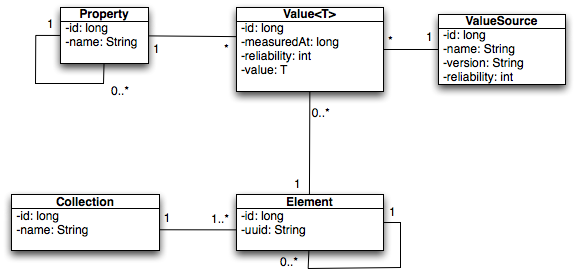
\includegraphics[width=5in]{figures/architecture/old_datamodel.png}
\caption{Old datamodel used in the first iteration.}
\label{fig:old_datamodel}
\end{center}
\end{figure}

\subsubsection{Core}
In the first implementation the controller worked in a single threaded, sequential manner due to simplicity reasons. However, preliminary experiments have shown that some tasks, such as meta data parsing make only partial use of the system resources at hand. For example the cpu utilisation was mostly less than 25\% during data parsing and storage. This was an indicator of a possible enhancement that might result in a significant speedup.

Because of the XML representation of the FITS meta data a parser had to be written in order to adapt the meta data schema of FITS to the internal data model. As FITS files usually are small in size (up to 5KB) the parser that was implemented utilised a DOM based approach. Early tests over a small set of FITS XML files seemed to have feasible performance. However, the first test over larger collections revealed the next issue: memory usage. Even though the amount of objects that had to be created by the DOM parser for each node in each xml document was not so high, the garbage collector of the JVM seemed to be unreliable and the overall consumption seemed to increase constantly with the xml document count and the collection size. This revealed the next potential optimisation.

C3PO's persistence layer was based on the Java Persistence API\footnote{http://docs.oracle.com/javaee/6/tutorial/doc/bnbpz.html} (JPA 1.0) with Hibernate\footnote{http://www.hibernate.org/} as the persistence provider in the first iteration. The higher level abstraction was done via a couple of generic data access object (DAO) interfaces, which were implemented by the client application, and client modules.

This design was chosen in order to allow each client application to choose its own implementation of the persistence layer. This was important since c3po is meant to be deployable in application server containers, that support the Java EE technology stack. For this, a special container managed transactional model would have been needed. On the other hand, content profiling is a data intensive process which can gain from the fact that the tool can execute near the data. That is why, also a local transactional model was needed, in which the tool should run locally near the data without any application server. All this would allow the separation of the data gathering and the data analysis parts of the work flow. The fact that the data base is external to the tool also means that it can be setup near the data or on a specific storage sever that has enough resources at its hand to handle the load.

Using an ORM framework, such as Hibernate is often very useful. However, in this instance a lot of optimisations and tweaks had to be done in order get out the most of the data base. While this was certainly possible, it was not the focus of the work to fight the framework. Using JVM profiling applications, revealed that a lot of resources are used during storage, because of the high volume of data and it seemed the ORM framework was the bottleneck.

\subsubsection{Applications}
In the first iteration only a prototype of the CLI application was implemented that made use of the non-transactional persistence model. It was used to measure performance and to monitor the behaviour of the whole framework. As far as the web application was concerned, only the persistence layer interfaces were implemented in order to validate the design and the separation of concerns.

\subsection{Second Iteration}
This section gives an overview of the implementation changes and enhancements in the second iteration and discusses the benefits and drawbacks of the alternatives.

\subsubsection{Data model}
After examination of the data at hand it seemed that the key value structure was fitting, but through the data base normalisation, performance was compromised. Thus, it seemed appropriate to exchange the underlying data source, which made it possible to remove the ORM framework at all. Its overhead was proven to be unnecessary during meta data adaptation and storage. Also, the analysis of the data seemed to take a unnecessary long time due to the many JOIN operations. One could argue that these could have been avoided by making the data model more specific, however this would have compromised the flexibility, which would have been a huge trade off.

For these reasons the data model was analysed again and different storage possibilities were evaluated.  Due to the natural key-value structure of the meta data it seemed that a key value store would possibly provide better solution to the problem. However, usually such solutions are used for caching (EHCache\footnote{http://ehcache.org}, Memchahed\footnote{http://memcached.org}, etc.) and architecture designers often have problems fitting their data model when such technologies are used for more than their purpose - caching. There are some implementations of data bases that offer most of the flexibility of the relational paradigm, high performance due to their almost key-value paradigm and out of the box horizontal scalability.

MongoDB\footnote{http://www.mongodb.org/} is a document store that uses BSON\footnote{http://bsonspec.org/} (Binary JSON) in order to store documents. These documents can have any kind of structure and do not have to be normalised in the relational database sense. On top of that MongoDB provides native facilities for executing Map Reduce \cite{Dean:2008:MSD:1327452.1327492} jobs on the server, which were proven to be very useful for aggregating and filtering the data. 

As any NoSQL solution, MongoDB does not gain from the fact that the data is normalised and relational. On the contrary, NoSQL solutions often give up normalisation in order to enhance performance of specific use cases. The data model from the first iteration was transformed into three collections (here the term collection is used in the sense of a document store and can be understood as the equivalent concept of a table in a relational database): one for the elements, one for the properties and one for the sources. The values are embedded into each element document and thus each document represents a self-contained object with all its known meta data - values, sources and conflicts. This has one big advantage when querying, as all values are already present without a need of joining the property table. Furthermore the equivalent of a SELECT statement in MongoDB does not retrieve the actual data, but only a cursor over it. This lazy-loading mechanism comes in handy in numerous use cases of the applications.
Figure \ref{fig:document_structure} gives an overview of the basic structure of element documents in BSON syntax. Note that the syntax is very similar to JSON, but provides data type support (e.g. the ObjectId).

\begin{figure}[h]
\begin{center}
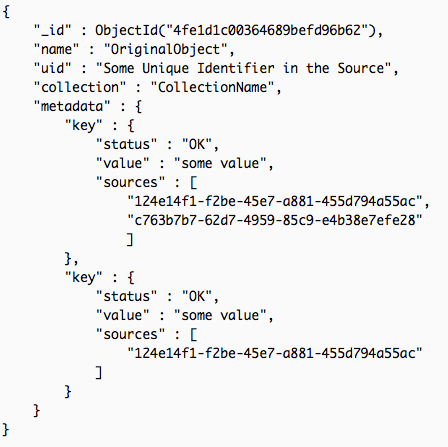
\includegraphics[width=4in]{figures/architecture/document_structure.png}
\caption{Structure of a c3po element in BSON.}
\label{fig:document_structure}
\end{center}
\end{figure}

Since Map-Reduce jobs are supported natively in MongoDB, it is easy to aggregate specific values of a specific keys in every element document or to execute some analysis queries. Another great advantage of this implementation is the pagination support. Every query in Mongo DB returns a cursor over the data, instead of the data itself. This makes navigation over the data within an application fast and efficient in terms of memory, as one does not have to consider the volume of the queried data.
The third reason, why Mongo was chosen, was the automatic load balancing used by the document store server. The document store supports horizontal scaling and auto node balancing out of the box, which might turn up useful when considering the amounts of data that the profiler has to deal with. To summarise MongoDB was chosen because of the:

\begin{itemize}
\item Natural fit of the data into a key-value schema
\item Native Map-Reduce support for data aggregation and near data processing
\item Query cursor and pagination
\item Horizontal scaling and automatic node balancing out of the box
\end{itemize}


\subsubsection{Core}
In the second iteration the controller and the meta data adaptors were reimplemented to follow a master-worker pattern.
The controller uses the gatherer interface to traverse the raw meta data files and spawns an adaptor worker thread for each file that has to be processed. This change resulted in much larger utilisation of CPU resources. Each meta data adaptor runs in a thread and is responsible for parsing meta data files that conform to a specific meta data schema. The c3po prototype makes use of a single adaptor for the FITS output format as described in (TODO cite). 

The parser implementation of the FITS adaptor was also changed due to the previous performance results. This time a SAX based approach was used. The Apache Commons Digester library\footnote{http://commons.apache.org/digester/} provides a special SAX parser that traverses each document only once and does not require the building of a complex DOM tree. This results in a much faster parsing with significantly less memory resources.

\subsubsection{Applications}
The CLI application was modified so that it reflects the changes of the new persistence layer.

Since the technology stack was different (no need of JAVA EE) and there was no need of transactional persistence model a new approach was also chosen for the web application. It makes use of a popular web application framework, called PlayFramework\footnote{http://playframework.org}, which does not rely on a complex technology, such as EJBs. It supports the developer to follow the MVC pattern and allows the rapid development of a REST \cite{Fielding:2000:ASD:932295} interface. REST was chosen for two main reasons. For one, it is easy to understand and pretty straightforward to implement. This allows easy integration with other tools, such as monitoring services (TODO cite) and a variety of client applications. The second reason is that other technologies, such as JavaServer Faces Technology\footnote{http://www.oracle.com/technetwork/java/javaee/javaserverfaces-139869.html} (JSF) and Enterprise Java Beans Technology\footnote{http://www.oracle.com/technetwork/java/javaee/ejb/index.html} (EJB) would have meant that only a few application servers will be compliant and able to support the application.
%REST cite: http://www.ics.uci.edu/~fielding/pubs/dissertation/rest_arch_style.htm

The UI was implemented with the help of the framework, by utilising Scala templates and standard technology such as HTML5, Javascript and CSS3. It enables the user to select her collection and obtain deeper overview by filtering the data based on specific properties and values as shown in figure \ref{fig:web_app_overview}.

\begin{figure}[htb]
\begin{center}
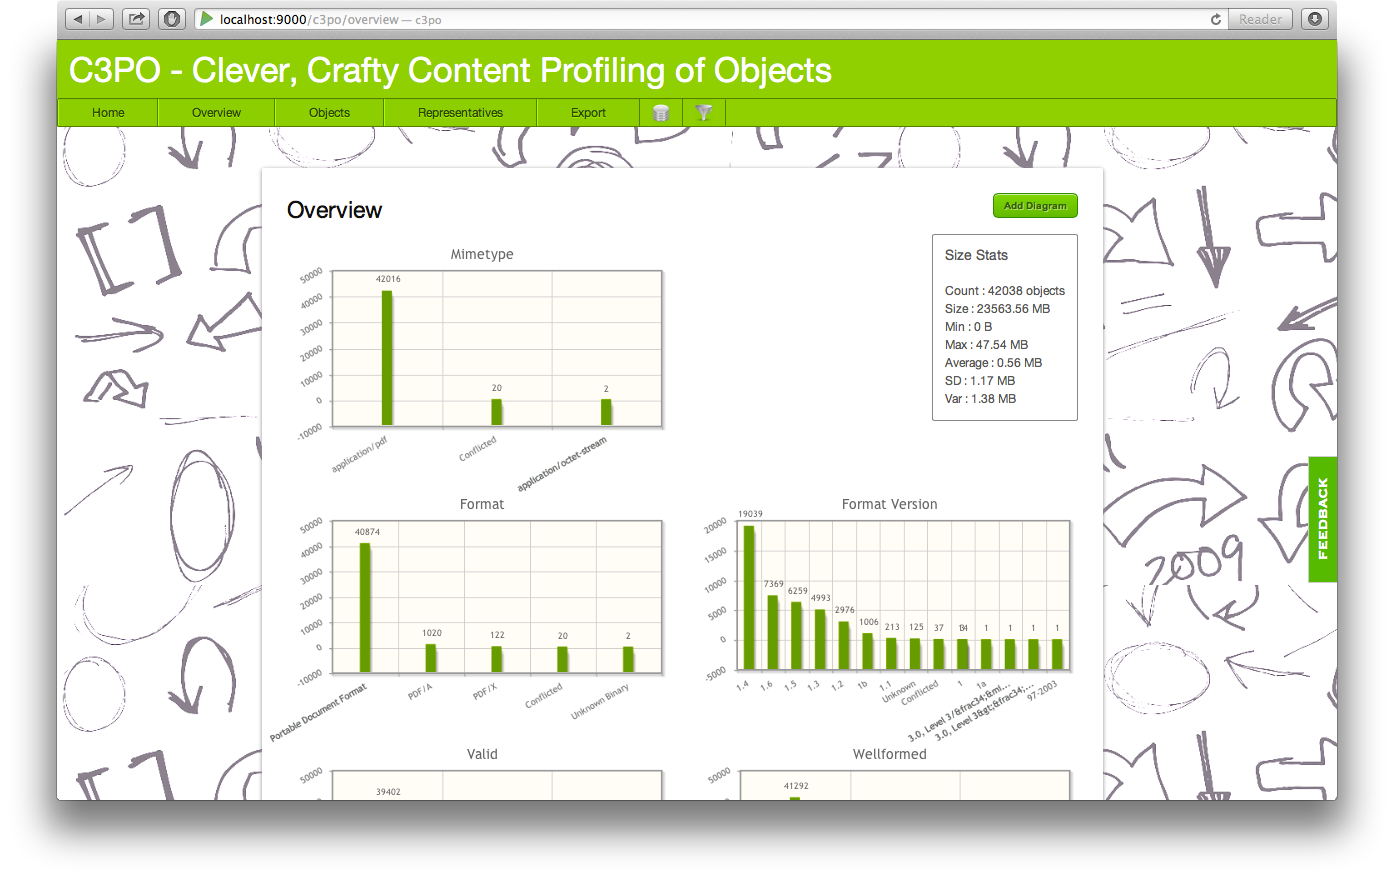
\includegraphics[width=5.5in]{figures/architecture/web_app_overview}
\caption{Screenshot of c3po - part of the overview of a collection.}
\label{fig:web_app_overview}
\end{center}
\end{figure}

\subsection{Comparison and Results}
Due to the changes made in the second iteration significant performance and scalability optimisations were achieved.

The change from a DOM to SAX parser not only improved the scalability of the system during gathering and parsing, but also improved the time for processing files. With the DOM solution in a single thread environment 1000 files were processed in about 3 minutes on average, whereas with the SAX solution 1000 files were processed in about 15 seconds.

In addition to the SAX parser enhancement the multi threading enhancement also showed promising results. With a single thread, parsing a collection consisting of about 1 Mio heterogeneous meta data files was done in about 165 minutes, whereas the same collection was processed on the same machine with 8 threads in about 104 minutes. This results in more than 35\% speedup just for parsing.

Other test results have shown that parsing and storing the raw meta data for a collection of about ~550 thousand files (web meta data) was done in about 17 minutes on a laptop, whereas the old solution needed about 12 hours for the same set of files on the same machine, due to the overhead of the ORM framework.

Furthermore, exporting a sparse matrix of all property values for every element in the collection was proven to be much faster. This was due to the fact, that the internal representation of the data needed no JOINS anymore and can be done by single iteration over a database cursor.

Many of the analysis queries were changed to be done by map-reduce jobs. Since these run near the data and not in the application itself, the scalability of such queries was significantly improved.

\subsection{Interfaces and Extension Points}
In order to extend the system, the framework provides a couple of interfaces. One important extension point for later use is the GathererInterface which provides an abstraction for the source of the raw meta data. It exposes a unified interface allowing the Controller to obtain streams to the next N files that have to be processed. This design allows a transparent view to the other modules in the system. The prototype of c3po provides an implementation only for local file systems. However, extending it to fetch data from a different source is just a matter of implementing a single interface, which is able to count the files to be processed and to open streams to the next N files. It is up to the implementing class to decide, whether the data will be retrieved over the network and the stream will be passed directly for further processing or it will be cached in batches to the local file system. Depending on the use case both could make sense and thus it is left in the responsibility of the service provider.

Clearly, meta data representation is another important aspect in such as system. For the prototype FITS was chosen, due to it benefits regarding normalisation and conflict detection. Nonetheless, other formats can make sense in specific use cases and when integrating with different sources, that utilise different meta data schemas. In order to extend c3po, one has to implement a simple adaptor that is able to parse the the new schema and return the data in a way that fits c3po's data model. A drawback here is that this will potentially break the property normalisation. For example two different meta data schemas can have two different property names with the same semantical meaning. There are a couple of solutions to this problem, which are taken into account in the design, but are not implemented due to insufficient information of real world scenarios. The first, could be to provide the mapping between these colliding properties via some user configuration and to take them into account during parsing or post-processing. The second solutions would be to allow the usage of a single adaptor based on the use case.

In order to obtain a profile, client applications can use the REST API. With a few simple calls a xml representation of a collection profile can be generated and retrieved. This file conforms to the proposed schema and provides simple aggregations of the data.
 
\section{Representative Sets}
Representative sets are one of the most important features of c3po, as they provide the basis for experiments during the planning phase. The selection of valid representatives can highly influence the decisions of a planner for the future of specific content. There are many different ways of selecting a small set of representatives.
Here we present a few algorithms that were implemented and discuss their benefits and drawbacks. It is important to keep in mind that real world scenarios can involve large collections of thousands to millions and even more digital objects, but usually the experiments during preservation planning are done on a very small set of representative sample objects in the order of 10 objects. 

\subsection{Random Selection}
As the  name suggests, this algorithm takes N random elements from the larger set and returns them. A simple pseudo code implementation looks like listing \ref{alg:random_selection}. Unfortunately, this approach is widely used in real world scenarios, due to the lack of automation support and understanding of the content at hand. One drawback of this approach is that it will most probably provide terrible results when applying it on a highly heterogenous content.
Nonetheless it could be useful in some cases, if the content is first filtered. For example, one can first apply some filters with C3PO and split the collection into smaller sets, that are homogeneous with respect to certain properties and then apply this algorithm on each of the subsets. If the smaller subsets are homogeneous enough, it is possible to achieve good results. Nonetheless, splitting and analysing the content could potentially take a lot of time.

\begin{algorithm}[H]
\SetAlgoLined
\SetKwFunction{RSS}{Random Sample Selection}
\SetKwInOut{Input}{Input}
\SetKwInOut{Output}{Output}

 \Input{A set of digital objects S and a upper limit N for the sample objects set}
 \Output{A set of random representative sample objects R}
 \BlankLine

\tcp{gets the number of objects in S}
count = \textit{S.size()}\; 
 
 \If{count $<=$ N} {
   \While{S.size() $!=$ 0} {
   \tcp{remove(i) removes and returns the object at index 'i'}
   	R.add(S.remove(0));
   }
 }
\Else{
 \While{R.size() $<=$ N} {
   \tcp{gets a pseudo random number between 0 and count}
   rand = getRandomNumber(count)\;
   \tcp{S[rand] get the object at index 'rand'}
   sample = S[rand]\;
   \tcp{add() appends the object to R}
   R.add(sample)\; 
  }
 }
 \caption{Random sample selection}
 \label{alg:random_selection}
\end{algorithm}

\subsection{Size Statistics}
This approach is probably the most common approach currently used by planners and preservation experts. It also selects random elements, however it considers some statistical information regarding the size of objects. This decision stems from the fact that preservation action tools often perform bad on objects with a large variation in size. Thus planners often take the smallest, largest and several average sized objects and conduct the experiments over them. If there are no other significant variations and differences in the objects, the selected representative set, could provide good results for planning. However, if the objects have significant variations in other characteristics other than the size, that might influence the preservation action tools, the algorithm would be error prone. A possible pseudo code implementation is provided in listing \ref{alg:size_selection}. Note that it makes use of a map reduce job that is executed near the data in order to calculate some statistics, such as the minimum, maximum, average and standard deviation, that are needed for the selection. The map, reduce and finalize functions, that make this aggregations possible are presented afterwards in javascript notation.

This approach is slightly better than the previous one, as it considers at least one characteristic of the meta data, that indeed often has influence on the experiments. If applied on a homogeneous set (with respect to the digital object type) it could give good results. Nonetheless, there are other factors that have to be considered. Especially in cases where the variance of the size in the collection is small.

\begin{algorithm}[H]
\SetAlgoLined
\SetKwFunction{SSS}{Size Statistics Sample Selection}
\SetKwInOut{Input}{Input}
\SetKwInOut{Output}{Output}

 \Input{A set of digital objects S and a upper limit N for the sample objects set}
 \Output{A set of random representative sample objects R}
 \BlankLine

\tcp{gets the number of objects in S}
count = \textit{S.size()}\; 
 
 \If{count $<=$ N} {
   \While{S.size() $!=$ 0} {
   \tcp{remove(i) remove and return the object at index 'i'}
   	R.add(S.remove(0));
   }
 }
\Else{
\tcp{map reduce job that calculates statistics for the property 'size'}
sizeStatistics = numericMapReduceJob('size')\;
min = sizeStatistics.getMin()\;
max = sizeStatistics.getMax()\;
avg = sizeStatistics.getAvg()\;
sd = sizeStatistics.getSd()\;
low = floor(avg - sd / 10)\;
high = ceil(avg - sd/10)\;
\BlankLine
minObject  = querySize(min)\;
maxObject = querySize(max)\;
A = querySizeBetween(low, high)\;
\BlankLine
R.add(minObject)\;
R.add(maxObject)\;
\BlankLine
\If{A.size() $>=$ (N-2)} {
  \While{R.size() $<$ N} {
    R.add(A.remove(0))\;
  }
}\Else{
  \While{A.size() $!=$ 0} {
   R.add(A.remove(0)\;
  }
}
}
 \caption{Size Statistics sample selection}
 \label{alg:size_selection}
\end{algorithm}


\begin{verbatim}

function map() {
  var size = this.metadata['size'].value;
  emit(1, {sum: size, min: size, max: size, count:1, diff: 0,});
}

function reduce(key, values) {
  var a = values[0];
  for (var i=1; i < values.length; i++){
    var b = values[i];
    var delta = a.sum/a.count - b.sum/b.count;
    var weight = (a.count * b.count)/(a.count + b.count);
    a.diff += b.diff + delta*delta*weight;
    a.sum += b.sum;a.count += b.count;
    a.min = Math.min(a.min, b.min);
    a.max = Math.max(a.max, b.max);
  }
  return a;
}

function finalize(key, value){
  value.avg = value.sum / value.count;
  value.variance = value.diff / value.count;
  value.stddev = Math.sqrt(value.variance);

  return value;
}
\end{verbatim}

\subsection{Systematic Sampling}
Systematic sampling is another optimisation of the random approach and is an equal-probability method. In other words it is more fair as every object in the set has equal probability to be chosen as a representative. It divides the content into 'n' buckets and calculates a 'skip' variable by dividing the number of objects in the population 'N' by the number of buckets 'n'. Then a random starting point is chosen between 0 and the calculated skip. Afterwards the next n-1 elements are chosen by adding the skip to the index of the last chosen element.  This will result in one element per bucket.
Even though this method is more fair, it still shows the same problems as the randoms sample selection algorithm. A pseudo code implementation is given in listing \ref{alg:systematic_sampling}

\begin{algorithm}[H]
\SetAlgoLined
\SetKwFunction{SSS}{Systematic Sampling Selection}
\SetKwInOut{Input}{Input}
\SetKwInOut{Output}{Output}

 \Input{A set of digital objects S and a upper limit N for the sample objects set}
 \Output{A set of random representative sample objects R}
 \BlankLine

\tcp{gets the number of objects in S}
count = \textit{S.size()}\; 
 
 \If{count $<=$ N} {
   \While{S.size() $!=$ 0} {  
   	R.add(S.remove(0));
   }
 }
\Else{
 limit = round(count / N)\;
 \tcp{generates a random number with a upper limit}
  skip = nextRandom(limit)\;
  
  \While{R.size() < N} {
     offset = skip * R.size() + skip\;
     R.add(S[offset])\;
  }
 }
 \caption{Systematic Sampling Selection}
 \label{alg:systematic_sampling}
\end{algorithm}

\subsection{Distribution Coverage}
The distribution coverage algorithm tries to find sample objects with the same distribution of the property value pairs of pre chosen characteristics. For example, if there is a collection consisting of 40\% PDF documents and 40\% Word documents and 20\% other documents and the sample set should be ten, then the algorithm will select 4 PDF files, 4 word files and 2 other files at random that are not PDF or Word documents.
If the user wants also other property value distributions taken into account, then these are also calculated. And the nearest distribution possible is returned.
This algorithm is better with respect to heterogeneity of properties within the same digital object type. It is also good in the sense that it does not consider the long tail of files, which is often good as these files usually have to be handled differently and are often responsible for messed up experiment results.

\section{Future Points of Interest}
There are many topics that can be handled and implemented in future work. Here we outline some and briefly discuss them:
\begin {itemize}
\item \textit{Scalability} is very important as the volumes of data will grow more and more over time. Even though the hardware resources and provided performance also grow over time the issue of scalability is very important. The authors believe that horizontal scalability is the best way to pursue. The current design decisions follow that path. More specifically, future enhancements should include the distributed map-reduce jobs and the caching of specific results, which will enhance the systems responsiveness.
\item \textit{Continous Profiling} is important as collections change over time. The support for including meta data of new and changed objects as well as adapting the computed aggregations in a easy, fast and scalable fashion is critical for the success of such an application in productuin use. Thus the investigation of the problems that arise with this will be important for future versions of the tool. The Map-Reduce facilities provide a potential solution to such a problem, since it is possible to aggregate new data and reuse old results, which are then just merged as the reduce function is always the same. 
\item \textit{Input to Digital Preservation Tools}. Monitoring systems and Simulators enhance the preservation planning processes by providing relevant and trustworthy information that is often hard to obtain due to its distribution and by offering simulations and projections of different outcomes based on current decisions and policies. Such systems heavily rely on larger amount of data. An integration with a content profile tool will play an important role for such tools as well as preservation planning activities.
\item \textit{Representative Sets} are the foundation for unbiased experiments and thus better performing algorithms in terms of speed and effective selection should be the focus of future work as well. 
\item \textit{Visualisation and Interactivity}. A wider variety of visualisations of different aspects of a collection can help and influence the decision of a user.
\end{itemize}

